\documentclass[11pt]{article}
\usepackage{fullpage}
\usepackage{url, graphicx}
\begin{document}
\thispagestyle{empty}
\parindent 0pt
\vfill
\large

\begin{center}
\LARGE{\bf \textsf{CS246: Mining Massive Datasets}}\\ {\bf \textsf{Homework 4}}
\\*[4ex]
\end{center}

\section*{Answer to Question 1(a)}
\begin{table}[h]
\centering
\label{my-label}
\begin{tabular}{|l|l|l|l|}
\hline
$w$                            & $w_1$& $w_2$& $w_3$\\ \hline
Initial                        & 0    & 0    & 0    \\
After Observing Patient ID = 1 & 0    & 0    & -1/5 \\
After Observing Patient ID = 2 & 0    & 0    & -1/5 \\
After Observing Patient ID = 3 & 0    & 0    & -1/5 \\
After Observing Patient ID = 4 & 0    & -1/5 & 0    \\
After Observing Patient ID = 5 & -1/5 & -1/5 & 1/5  \\ \hline
\end{tabular}
\end{table}

\pagebreak[4]
\section*{Answer to Question 1(b)}
The Perceptron algroithm will not return a solution to those data.
Those data points are not linearly seperable.

\begin{figure}[h]
\center
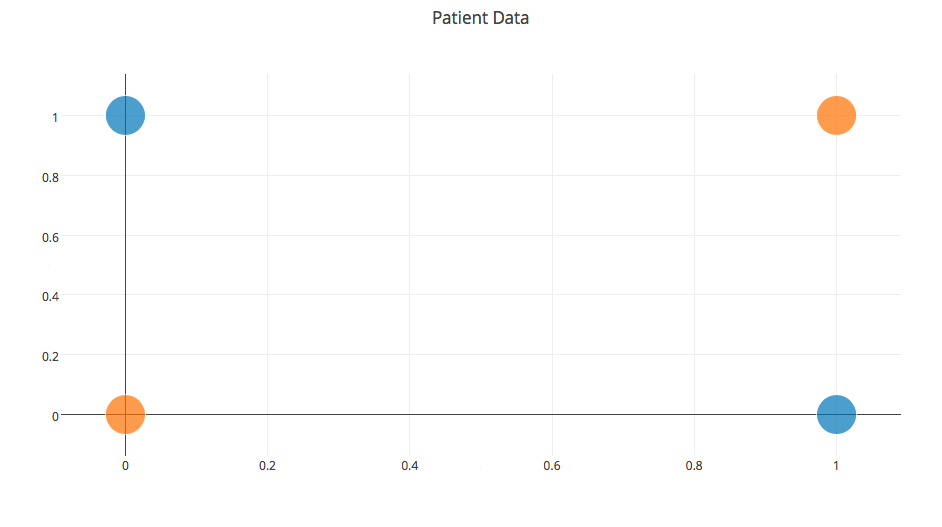
\includegraphics[scale=0.4]{patientData.png}
\caption{Patient Data}
\end{figure}

\pagebreak[4]
\section*{Answer to Question 1(c)}
From below figures it is found that only $\psi=((\phi_1 xor \phi_2),\phi_2,−1)$ is linear seperable.
The associated $w = (-1, 0, -0.5)$
\begin{figure}[h]
\center
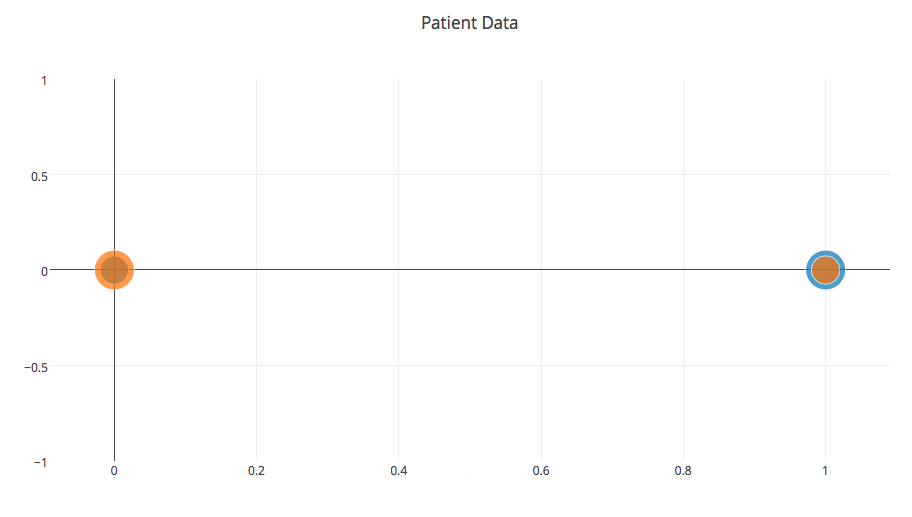
\includegraphics[scale=0.2]{patientData1.png}
\caption{$\psi = (\phi_1^2, \phi_1\phi_2, −1)$}
\end{figure}

\begin{figure}[h]
\center
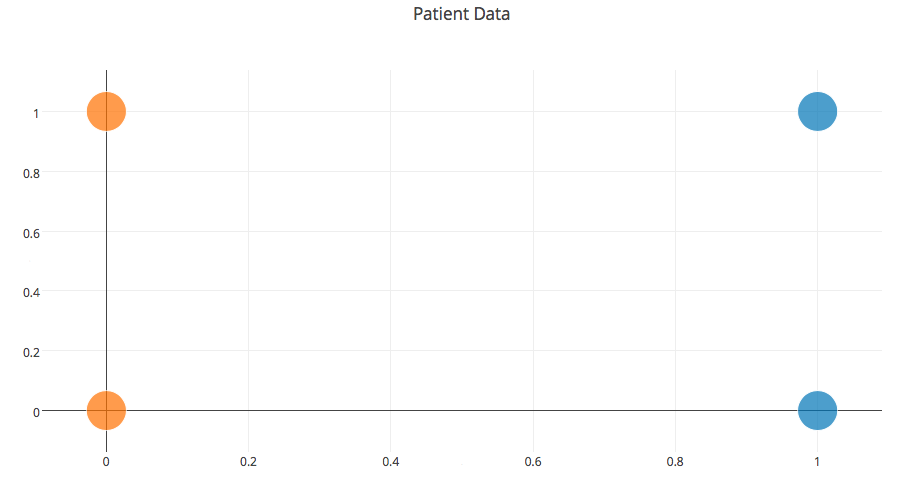
\includegraphics[scale=0.2]{patientData2.png}
\caption{$\psi=((\phi_1 xor \phi_2),\phi_2,−1)$}
\end{figure}

\begin{figure}[h]
\center
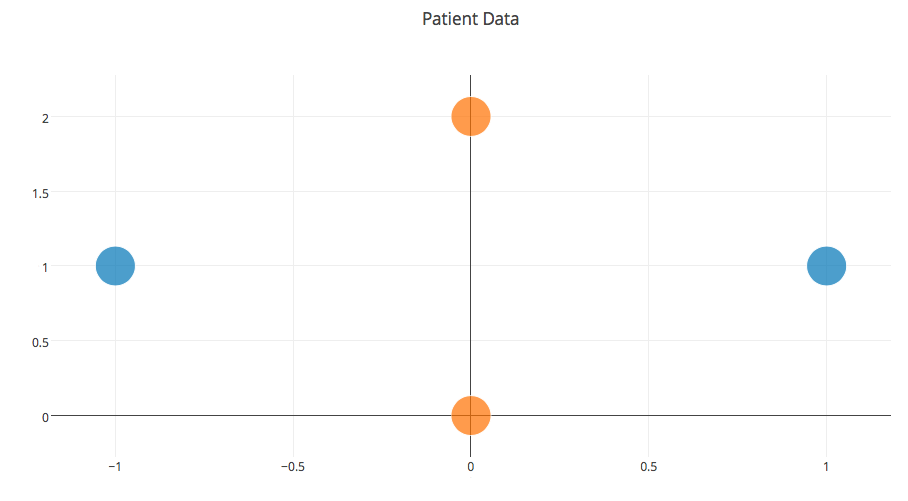
\includegraphics[scale=0.2]{patientData3.png}
\caption{$\psi=(\phi_1 - \phi_2,\phi_1 + \phi_2,−1)$}
\end{figure}



\pagebreak[4]
\section*{Answer to Question 2(a)}

\pagebreak[4]
\section*{Answer to Question 2(b)}

\pagebreak[4]
\section*{Answer to Question 3(a)}

\pagebreak[4]
\section*{Answer to Question 3(b)}

\pagebreak[4]
\section*{Answer to Question 4(a)}

\pagebreak[4]
\section*{Answer to Question 4(b)}

\pagebreak[4]
\begin{center}
\LARGE{\bf \textsf{Cover Sheet}} \\*[4ex]
\end{center}

\textbf{Assignment Submission } Fill in and include this cover sheet with each of your assignments. Assignments are due at 11:59pm. All students (SCPD and non-SCPD) must submit their homeworks via GradeScope (\url{http://www.gradescope.com}). Students can typeset or scan their homeworks. Make sure that you answer each question on a separate page. Students also need to upload their code at \url{http://snap.stanford.edu/submit}. Put all the code for a single question into a single file and upload it. Please do not put any code in your GradeScope submissions.
\\
\\
\textbf{Late Day Policy } Each student will have a total of {\em two} free late periods. {\em One late period expires at the start of each class.} (Homeworks are usually due on Thursdays, which means the first late periods expires on the following Tuesday.) Once these late periods are exhausted, any assignments turned in late will be penalized 50\% per late period. However, no assignment will be accepted more than {\em one} late period after its due date.
\\
\\
\textbf{Honor Code } We strongly encourage students to form study groups. Students may discuss and work on homework problems in groups. However, each student must write down their solutions independently i.e., each student must understand the solution well enough in order to reconstruct it by him/herself.  Students should clearly mention the names of all the other students who were part of their discussion group. Using code or solutions obtained from the web (github/google/previous year solutions etc.) is considered an honor code violation. We check all the submissions for plagiarism. We take the honor code very seriously and expect students to do the same.

\vfill
\vfill

{\Large
\textbf{Your name:} \hrulefill \\
\textbf{Email:} \underline{\hspace*{7cm}} \textbf{SUID:} \hrulefill\\*[2ex] }
Discussion Group (People with whom you discussed ideas used in your answers): \\\\\\
On-line or hardcopy documents used as part of your answers: \\\\\\
\vfill

\vfill

I acknowledge and accept the Honor Code.\\*[3ex]
\bigskip
\textit{(Signed)}\hrulefill
% If you are not printing this document out, just type your initials above

\vfill
\vfill

\end{document}

